This chapter describes the implementation of the hybrid FAIRness
assessment framework introduced in Chapter~3. It explains how the
proposed design is realized as a modular software pipeline, covering
repository data collection, deterministic rule-based assessment,
LLM-based documentation assessment, and hybrid profile generation.
The chapter also presents the web-based prototype developed to expose
the assessment results, support comparison of the evaluated LLM
configurations, and enable interactive assessment of public GitHub
repositories. Finally, implementation-specific limitations of the
prototype are discussed.

\section{System Architecture and Overview}

The proposed framework is implemented as a modular assessment pipeline
of independent Python components organized around four main processing
stages: repository data collection, rule-based assessment, LLM-based
assessment, and hybrid profile generation. A web-based application
layer is implemented on top of this pipeline to expose saved assessment
results and to support assessment of newly supplied public GitHub
repositories.

The core processing components exchange data primarily through files
stored on the local filesystem rather than through a shared database.
This organization allows individual stages to be executed, inspected,
and re-run independently, while the web application reuses the same
assessment logic for interactive access to the framework. Where
appropriate, batch-processing stages also include mechanisms for
skipping already processed repositories, reducing unnecessary repeated
work after interruption.

The implementation is written in Python. GitHub repository data is retrieved 
through the GitHub REST API using the \texttt{requests} library, while LLM 
inference is performed through a locally running Ollama instance for the primary 
Llama configuration and through a remote OpenAI-compatible API for the second model 
configuration described in Section~4.4. Standard file formats, primarily JSON and CSV, 
are used to persist intermediate and final results. Repository data is
stored as per-repository snapshots containing the README content,
general GitHub metadata, and an inventory of FAIR-related files.
This file-based representation makes the evidence used by subsequent
assessment stages directly inspectable and allows the scoring
components to operate on previously collected snapshots without
re-querying GitHub.

The overall data flow consists of four stages, illustrated in
Figure~\ref{fig:system_architecture}

\begin{figure}[htbp]
    \centering
    \begin{tikzpicture}[
    node distance=1.0cm and 1.2cm,
    box/.style={
        draw,
        rounded corners,
        rectangle,
        align=center,
        minimum height=1.15cm,
        text width=5.0cm,
        font=\small
    },
    smallbox/.style={
        draw,
        rounded corners,
        rectangle,
        align=center,
        minimum height=1.15cm,
        text width=4.5cm,
        font=\small
    },
    arrow/.style={
        -{Latex[length=2.5mm]},
        thick
    }
]

% GitHub
\node[box] (github) {
    \textbf{GitHub}\\
    Repository Search and REST API
};

% Collection
\node[box, below=of github] (collection) {
    \textbf{Repository Collection and Filtering}\\
    Topic search, filtering, deduplication,
    metadata and README retrieval
};

% Snapshot
\node[box, below=of collection] (snapshot) {
    \textbf{Local Repository Snapshot}\\
    README content\\
    \texttt{metadata.json}\\
    \texttt{fair\_file\_checks.json}
};

% Rule branch
\node[smallbox, below left=1.4cm and 0.8cm of snapshot] (rule) {
    \textbf{Rule-Based Assessment}\\
    F1--R2\\
    Six binary structural indicators
};

% LLM branch
\node[smallbox, below right=1.4cm and 0.8cm of snapshot] (llm) {
    \textbf{LLM-Based Assessment}\\
    D1--D6\\
    Scores, confidence and reasoning
};

% Rule output
\node[smallbox, below=of rule] (ruleout) {
    \textbf{Rule-Based Results}\\
    CSV output
};

% LLM output
\node[smallbox, below=of llm] (llmout) {
    \textbf{LLM Results}\\
    Parsed CSV + raw/JSON outputs
};

% Hybrid
\node[box, below=2.0cm of snapshot, yshift=-4.0cm] (hybrid) {
    \textbf{Hybrid FAIRness Profile Generator}\\
    Join assessment outputs by repository identifier
};

% Final profile
\node[box, below=of hybrid] (profile) {
    \textbf{Repository FAIRness Profile}\\
    F1--R2 structural indicators\\
    D1--D6 documentation scores\\
    Confidence and reasoning
};

% Arrows
\draw[arrow] (github) -- (collection);
\draw[arrow] (collection) -- (snapshot);

\draw[arrow] (snapshot.south) |- (rule.north);
\draw[arrow] (snapshot.south) |- (llm.north);

\draw[arrow] (rule) -- (ruleout);
\draw[arrow] (llm) -- (llmout);

\draw[arrow] (ruleout.south) |- (hybrid.west);
\draw[arrow] (llmout.south) |- (hybrid.east);

\draw[arrow] (hybrid) -- (profile);

\end{tikzpicture}
     \caption{Processing flow of the implemented hybrid FAIRness assessment pipeline.}
    \label{fig:system_architecture}
\end{figure}

First, the collection component retrieves and prepares repository
information from GitHub, producing the local repository snapshots used
as input to subsequent stages. Second, the rule-based component
evaluates structural evidence and produces six binary indicators
(F1--R2). Third, the LLM-based documentation component processes README documentation
and produces six ordinal documentation scores (D1--D6), each
accompanied by a confidence label and a short reasoning statement.
Finally, the hybrid profile generation component joins the structural
and documentation-based outputs by repository identifier and stores
them as a unified repository profile while preserving the two
assessment components as separate dimensions.

The rule-based assessment was executed for the complete
188-repository dataset. LLM assessment was executed for the
30-repository ground-truth corpus used for manual evaluation, and
hybrid profiles were consequently generated for repositories for
which both rule-based and LLM-based results were available. The implemented components therefore cover all stages required to
construct the hybrid profile, while the experimental execution of the
LLM-based component is restricted to the annotated evaluation corpus.

In addition to the batch-processing workflow used for the empirical
evaluation, the implemented framework provides a web-based interface
for inspecting saved assessment results and applying the assessment
procedure to a newly supplied public GitHub repository. The web layer
is implemented using FastAPI and a lightweight HTML, CSS, and
JavaScript frontend. It reuses the existing assessment components
rather than implementing a separate scoring procedure. Saved thesis
results and newly generated live assessments are kept distinct so that
interactive use of the prototype does not modify the fixed datasets
used for the empirical evaluation.

\section{Repository Data Collection and Local Representation}

Repository data collection is implemented as a two-phase process:
repository discovery and selection, followed by per-repository data
retrieval. Both phases interact with the GitHub REST API and are
implemented as separate Python components. Repository discovery
constructs the initial dataset, whereas the retrieval stage operates
on the resulting repository list to obtain the artefacts required by
the subsequent assessment components.

Repository discovery queries GitHub for repositories associated with
the research domains defined during dataset construction. Candidate
repositories are deduplicated by their GitHub repository identifier
and filtered according to the inclusion and exclusion criteria
described in Chapter~3. These criteria remove repositories that do not
meet the intended characteristics of the research software dataset,
including repositories identified as forks, archived projects, and
repositories matching predefined exclusion conditions. The resulting
repository list is persisted in machine-readable form and subsequently
processed by the data retrieval stage.

For each selected repository, the retrieval component obtains three
main types of information. First, README content is retrieved through
GitHub's dedicated README endpoint and stored locally for subsequent
documentation assessment. Second, the repository metadata returned by
the GitHub repository endpoint is stored in a \texttt{metadata.json}
file. This record contains the GitHub metadata required by later
processing stages, including repository and licensing information.
Third, the contents of the repository root are queried and compared
against a predefined set of FAIR-related filenames. The resulting
presence inventory is stored as
\texttt{fair\_file\_checks.json}. Candidate files include README and
license variants, citation and structured metadata files, dependency
specifications, and contribution files.

The collected artefacts are organized as local repository snapshots.
Each repository is assigned a directory based on its owner and
repository name, containing the retrieved README, repository metadata,
and FAIR-related file inventory. This representation decouples data
collection from assessment: once a snapshot has been created, the
rule-based and LLM-based components can operate on the locally stored
evidence without repeatedly querying GitHub. It also makes the exact
repository evidence used during an assessment directly inspectable.

The full-dataset retrieval implementation includes basic support for
resuming interrupted collection runs. Before retrieving a repository,
the collector checks whether a local \texttt{metadata.json} file
already exists and, if so, skips that repository. This avoids repeated
API requests for repositories treated as previously collected, although
the presence of this file is used as the completion marker and the
collector does not independently verify that every expected snapshot
artefact is present. The ground-truth collection workflow does not use
the same repository-level skip mechanism. The resulting snapshots form
the common input representation used by the subsequent assessment
components.

\section{Rule-Based Assessment Implementation}

The rule-based assessment component evaluates each repository
snapshot against the six binary FAIR indicators (F1--R2) defined in
Chapter~3, operating exclusively on the locally stored README,
metadata, and file-inventory artefacts produced by the collection
stage; no GitHub API access occurs during scoring.

Each indicator is implemented as an independent boolean check,
drawing on one or more of three evidence sources: the precomputed
file-presence inventory, the stored GitHub metadata record, and the
README text itself. F2 (Structured Metadata) is evaluated by
checking for recognized metadata filenames using both the stored
file-presence inventory and the local repository snapshot. R1
(README Present) directly checks the snapshot for one of the
recognized README filename variants. I1 (Dependency Specification)
similarly evaluates recognized dependency and build files across
multiple programming-language ecosystems. F1 (Persistent Identifier)
searches the README together with any locally stored
\texttt{CITATION.cff} and \texttt{codemeta.json} content for patterns
associated with common persistent identifier formats, including
doi.org URLs, Zenodo record and badge links, and Software Heritage
identifiers. A1 (License) reflects the three evidence sources
described in Chapter~3: a recognized license filename, a license
field in the stored GitHub metadata, or explicit licensing language
in the README text; the three sources are checked in this order, so
that structured evidence takes precedence and README text is only
relied upon when no file or metadata evidence is found. R2 (Citation
Information) is satisfied either by the presence of a dedicated
citation file or by matching one of several phrasings commonly used
to request citation of a software project within the README text.

Where file-presence evidence is required, the implementation does
not rely solely on the precomputed inventory. The corresponding path
in the local repository snapshot is also checked, allowing a
file-based indicator to be satisfied when the artefact exists locally
but is absent from the stored presence record.

The scorer processes repositories in batch, reading each
repository's snapshot folder in turn and producing a single
six-indicator vector per repository, together with an aggregated
rule-based total ranging from 0 to 6. Repositories whose snapshot is
incomplete --- for example, missing the metadata or file-inventory
record --- are skipped and reported rather than scored with
incomplete evidence. Results are written to a single CSV file, with
one row per repository, in which each of the six indicators and the
aggregated total form separate columns. This output format is shared
by both the full 188-repository dataset run and the 30-repository
ground truth validation run.


\section{LLM-Based Assessment Implementation}
The LLM-based assessment component evaluates README documentation
against the six documentation quality dimensions (D1--D6) defined in
Chapter~3. Two model configurations are supported: Llama~3.1~8B
through a locally running Ollama instance and
\texttt{Qwen3.6-35B-A3B-MLX-8bit} through the university KISTE
service using an OpenAI-compatible API.

The two implementations share the same substantive assessment rubric,
README-only evidence boundary, and 12,000-character input limit, while
provider-specific request and response handling is implemented
separately.

For each repository, the README is located by checking a fixed set
of recognized filenames in priority order, so that non-Markdown
README variants are still picked up if present. The retrieved text
is truncated to the first 12{,}000 characters where it exceeds this
length, consistent with the preprocessing limit described in
Chapter~3, before being inserted into a fixed prompt template
together with the repository name. The prompt instructs the model to score each of the six dimensions
according to the rubric criteria and to base each score only on evidence
explicitly present in the README text. Both model configurations return
a score, confidence label (HIGH, MEDIUM, or LOW), and reasoning field
for each dimension. The Qwen prompt additionally requests a concise
one-sentence justification, while the Llama implementation requires the
reasoning field through its structured response schema.

For the primary Llama~3.1~8B configuration, the scorer submits each
request to Ollama's HTTP API rather than invoking the model through a
command-line interface. The sampling temperature is set to zero, and a
structured JSON schema is supplied as part of the request. The schema
constrains the response to the six required dimensions, restricts each
score to the integer values 0, 1, or 2, and restricts each confidence
label to one of the three permitted values.

On receiving a response, the Llama implementation performs an
additional validation pass independent of the schema, confirming that
all six dimensions are present and that every score and confidence
value falls within the expected range before accepting the result. If
a response is missing, malformed, or fails this validation, the request
is retried once; if the retry also fails, the repository is recorded
as failed and scoring proceeds to the next repository rather than
halting the batch run.

Nonempty raw model responses are persisted before parsing, preserving
the original output returned by the model service for later inspection,
including responses that subsequently fail parsing or validation.
Attempts that return no response, or fail before a model response is
received, do not produce a raw-response file. For successfully scored
repositories, the parsed and validated JSON representation is stored
separately.

Batch execution is resumable at the level of individual repositories.
Before submitting a repository for assessment, the implementation
checks whether a previously parsed result is already available and
skips repositories that have already been successfully processed.
This allows interrupted runs to continue without repeating completed
LLM inference.

Successfully scored repositories are appended incrementally to a
single CSV output file as they complete, with one row per repository
containing the score, confidence level, and reasoning text for each
of the six dimensions, together with the model name and a timestamp.
This output format matches the one described in Chapter~3 and is
applied to all 30 ground truth repositories.

A second LLM-based scorer implementation targets Qwen3.6-35B-A3B-MLX-8bit, 
accessed through an OpenAI-compatible chat completion API hosted on a remote 
GPU server rather than through the local Ollama instance. This implementation 
reuses the same dimension definitions, substantive prompt structure, and rubric described above, 
adapted only where required by the different backend: structured output is obtained 
through explicit prompt instructions combined with post-hoc JSON validation rather than 
a server-enforced schema, and the model's separately returned reasoning trace is discarded 
before scoring. Results are written to per-model output files following the same schema as the 
Llama-based output, so that the two models' results can be compared directly without either overwriting 
the other.
 \section{Hybrid Profile Generation}

The hybrid profile generation component combines the outputs of the
rule-based and LLM-based components into a single unified record per
repository, without computing any combined or weighted score.

The component reads the rule-based and LLM-based result CSV files
produced by the two preceding stages and indexes each by repository
identifier. This process is repeated independently for each evaluated 
LLM configuration, producing one hybrid profile set per model, each 
generated by joining the shared rule-based results with that model's 
LLM-based results. An inner join is then performed between the two sets of
results, so that a hybrid profile is produced only for repositories
present in both inputs. Because the LLM-based component was applied
only to the 30-repository ground truth corpus, this join
consequently restricts the set of generated hybrid profiles to those
repositories, even though rule-based results exist for the complete
188-repository dataset.

For each matched repository, the resulting record concatenates the
six rule-based indicator scores (F1--R2) and the aggregated
rule-based total with the six LLM-based dimension scores (D1--D6),
each accompanied by its confidence level and reasoning text, the
aggregated LLM total, and the model name and timestamp associated
with the LLM assessment. No arithmetic combination or weighting is
applied across the two sets of scores at any point in this process;
the structural and documentation-based dimensions are retained as
distinct fields within the same record, consistent with the design
rationale described in Chapter~3. A single timestamp is recorded for
the batch as a whole, and repositories are written in a fixed,
sorted order to ensure that the output is deterministic regardless
of the order in which the two input files were produced.

The combined records are written to a single CSV file, with one row
per repository, representing the hybrid FAIRness profile produced by
the proposed framework. The profile provides a unified representation
of the structural and documentation-based assessment results while
preserving their distinct scoring schemes.

\section{Example Repository Profile}

To illustrate the output produced by the framework, this section
presents the complete hybrid FAIRness profile generated for
\texttt{astropy/astropy}, one of the 30 ground truth repositories.
This repository was selected because its profile shows a clear
contrast between the two assessment components: it achieves the
maximum possible rule-based score while receiving a comparatively
low LLM-based documentation score, illustrating the kind of gap
that a purely structural assessment would not reveal.

\subsection{Rule-Based Indicators}

Table~\ref{tab:example_rule} shows the six rule-based indicator
scores produced for this repository.

\begin{table}[h]
\centering
\caption{Rule-based indicator scores for \texttt{astropy/astropy}.}
\label{tab:example_rule}
\begin{tabular}{lc}
\hline
\textbf{Indicator} & \textbf{Score} \\
\hline
F1 --- Persistent Identifier    & 1 \\
F2 --- Structured Metadata      & 1 \\
A1 --- License                  & 1 \\
I1 --- Dependency Specification & 1 \\
R1 --- README Present           & 1 \\
R2 --- Citation Information     & 1 \\
\hline
\textbf{Rule-based total}       & \textbf{6 / 6} \\
\hline
\end{tabular}
\end{table}

The repository satisfies all six structural indicators, reflecting
the presence of a persistent identifier, a structured metadata file,
a recognized license, a dependency specification file, a README, and
explicit citation information.

It is important to note that this assessment is restricted to evidence
contained directly in the README. The Astropy README links to extensive
external documentation that provides additional installation, usage,
and dependency information; however, the content behind these links is
not retrieved by the implemented LLM assessment pipeline. Consequently,
the scores in Table~\ref{tab:example_llm} should be interpreted as an
assessment of the documentation evidence available directly in the
README, rather than of the overall quality or completeness of Astropy's
documentation.

\subsection{LLM-Based Documentation Dimensions}
Table~\ref{tab:example_llm} shows the documentation-quality assessment
produced by the primary Llama~3.1~8B configuration for
\texttt{astropy/astropy}, together with the confidence level and
reasoning associated with each dimension.
\begin{table}[h]
\centering
\caption{Llama~3.1~8B documentation assessment for
\texttt{astropy/astropy}.}
\label{tab:example_llm}
\small
\begin{tabular}{lccp{8cm}}
\hline
\textbf{Dimension} & \textbf{Score} & \textbf{Confidence} & \textbf{Reasoning} \\
\hline

D1 --- Installation
  & 0
  & HIGH
  & The README provides only a single line of installation
    information (\texttt{pip install astropy}), without mentioning
    required prerequisites. \\

D2 --- Usage
  & 0
  & HIGH
  & There is no concrete command, code snippet, workflow, or
    executable example in the README to demonstrate how to use the
    software. \\

D3 --- Purpose
  & 1
  & MEDIUM
  & The README explains that Astropy is a community effort to
    develop a single core package for astronomy in Python, but it
    does not clearly explain its intended domain or audience. \\

D4 --- Dependencies
  & 0
  & HIGH
  & There is no information about required and/or optional
    dependencies provided in human-readable form in the README. \\

D5 --- Examples
  & 1
  & MEDIUM
  & The README mentions GitHub Codespaces as a way to start
    developing Astropy, but it does not contain a meaningful usage
    example, nor explicitly link to an example gallery or tutorial
    demonstrating software use. \\

D6 --- Contribution
  & 2
  & HIGH
  & The README provides contribution guidance and at least one
    support or community channel (Slack), as well as multiple ways
    to contribute, including code submission, feedback, and
    documentation updates. \\
\hline
\multicolumn{3}{l}{\textbf{LLM total}} & \textbf{4 / 12} \\
\hline
\end{tabular}
\end{table}

The confidence label reflects the model's self-reported confidence in
the assigned score itself, independent of whether that score is low or
high: a HIGH label on D1 indicates high confidence in assigning a low
score because installation information is lacking, just as the HIGH
label on D6 indicates high confidence in assigning a high score because
the contribution guidance is present and complete.

\subsection{Profile Representation}

The example illustrates how the implemented hybrid profile preserves
the outputs of the two assessment components separately. The
rule-based component assigns positive values to all six implemented
structural indicators, resulting in a total of 6/6. The Llama-based
component produces a documentation total of 4/12, together with
dimension-specific scores, confidence labels, and reasoning.

These documentation values represent the output generated by the
implemented LLM assessment pipeline rather than independently validated
judgements of documentation quality. In particular, the profile
preserves the model's original criterion-level decisions even where
their correspondence with the annotation rubric requires further
evaluation.

The example therefore demonstrates the representation produced by the
hybrid implementation: structural evidence and LLM-based documentation
assessment are available for the same repository without being
collapsed into a single overall FAIRness score. The correctness and
reliability of these outputs relative to the manual annotations are
evaluated separately in Chapter~5.

\section{Web-Based Assessment Interface}

\subsection{Web Application Architecture}

To make the assessment results inspectable and to demonstrate the
framework beyond batch-generated CSV files, a web-based prototype was
implemented on top of the assessment pipeline. The application uses a
FastAPI backend together with a lightweight frontend implemented in
HTML, CSS, and JavaScript.

The web layer does not introduce an alternative assessment procedure.
Instead, it reuses the same rule-based and LLM-based scoring logic used
by the batch-processing pipeline. The backend provides access to the
saved thesis results and coordinates live repository assessment, while
the frontend presents the resulting structural and documentation-based evidence in an interactive form.

The application distinguishes between two result sources. Saved thesis
assessments correspond to the fixed datasets used in the empirical
study, whereas live assessments are generated from the current content
of a user-supplied public GitHub repository. Live assessments are not
written into the fixed thesis dataset and therefore do not alter the
results evaluated in Chapter~5.

\subsection{Dataset Overview}

The overview view provides an aggregate representation of the saved
assessment results. Structural evidence is summarized across the full
dataset of 188 repositories, while documentation-quality results are
reported for the 30-repository annotated corpus on which the LLM-based
assessment was executed. The interface explicitly distinguishes these
two populations to avoid implying that documentation scores are
available for all 188 repositories.

Because documentation assessments were generated separately for the
two evaluated LLM configurations, the interface allows the displayed
saved documentation results to be selected by model. Changing this
selection affects the documentation summaries and repository-level
documentation results, while the deterministic structural assessment
remains unchanged. Model selection is exposed primarily to support
transparent inspection of model-dependent assessment behaviour rather
than to imply that the two configurations are interchangeable.

The overview reports the prevalence of the six structural indicators,
the distribution of structural totals, and the mean scores of the six
README documentation dimensions for the selected model configuration.
Structural and documentation results remain visually separated and are
not combined into an overall FAIRness score, following the
hybrid-profile design described in Chapter~3.

Figure~\ref{fig:web_overview} shows the resulting dataset overview for
the two evaluated documentation model configurations.

\begin{figure}[p]
    \centering

    \begin{subfigure}{\textwidth}
        \centering
        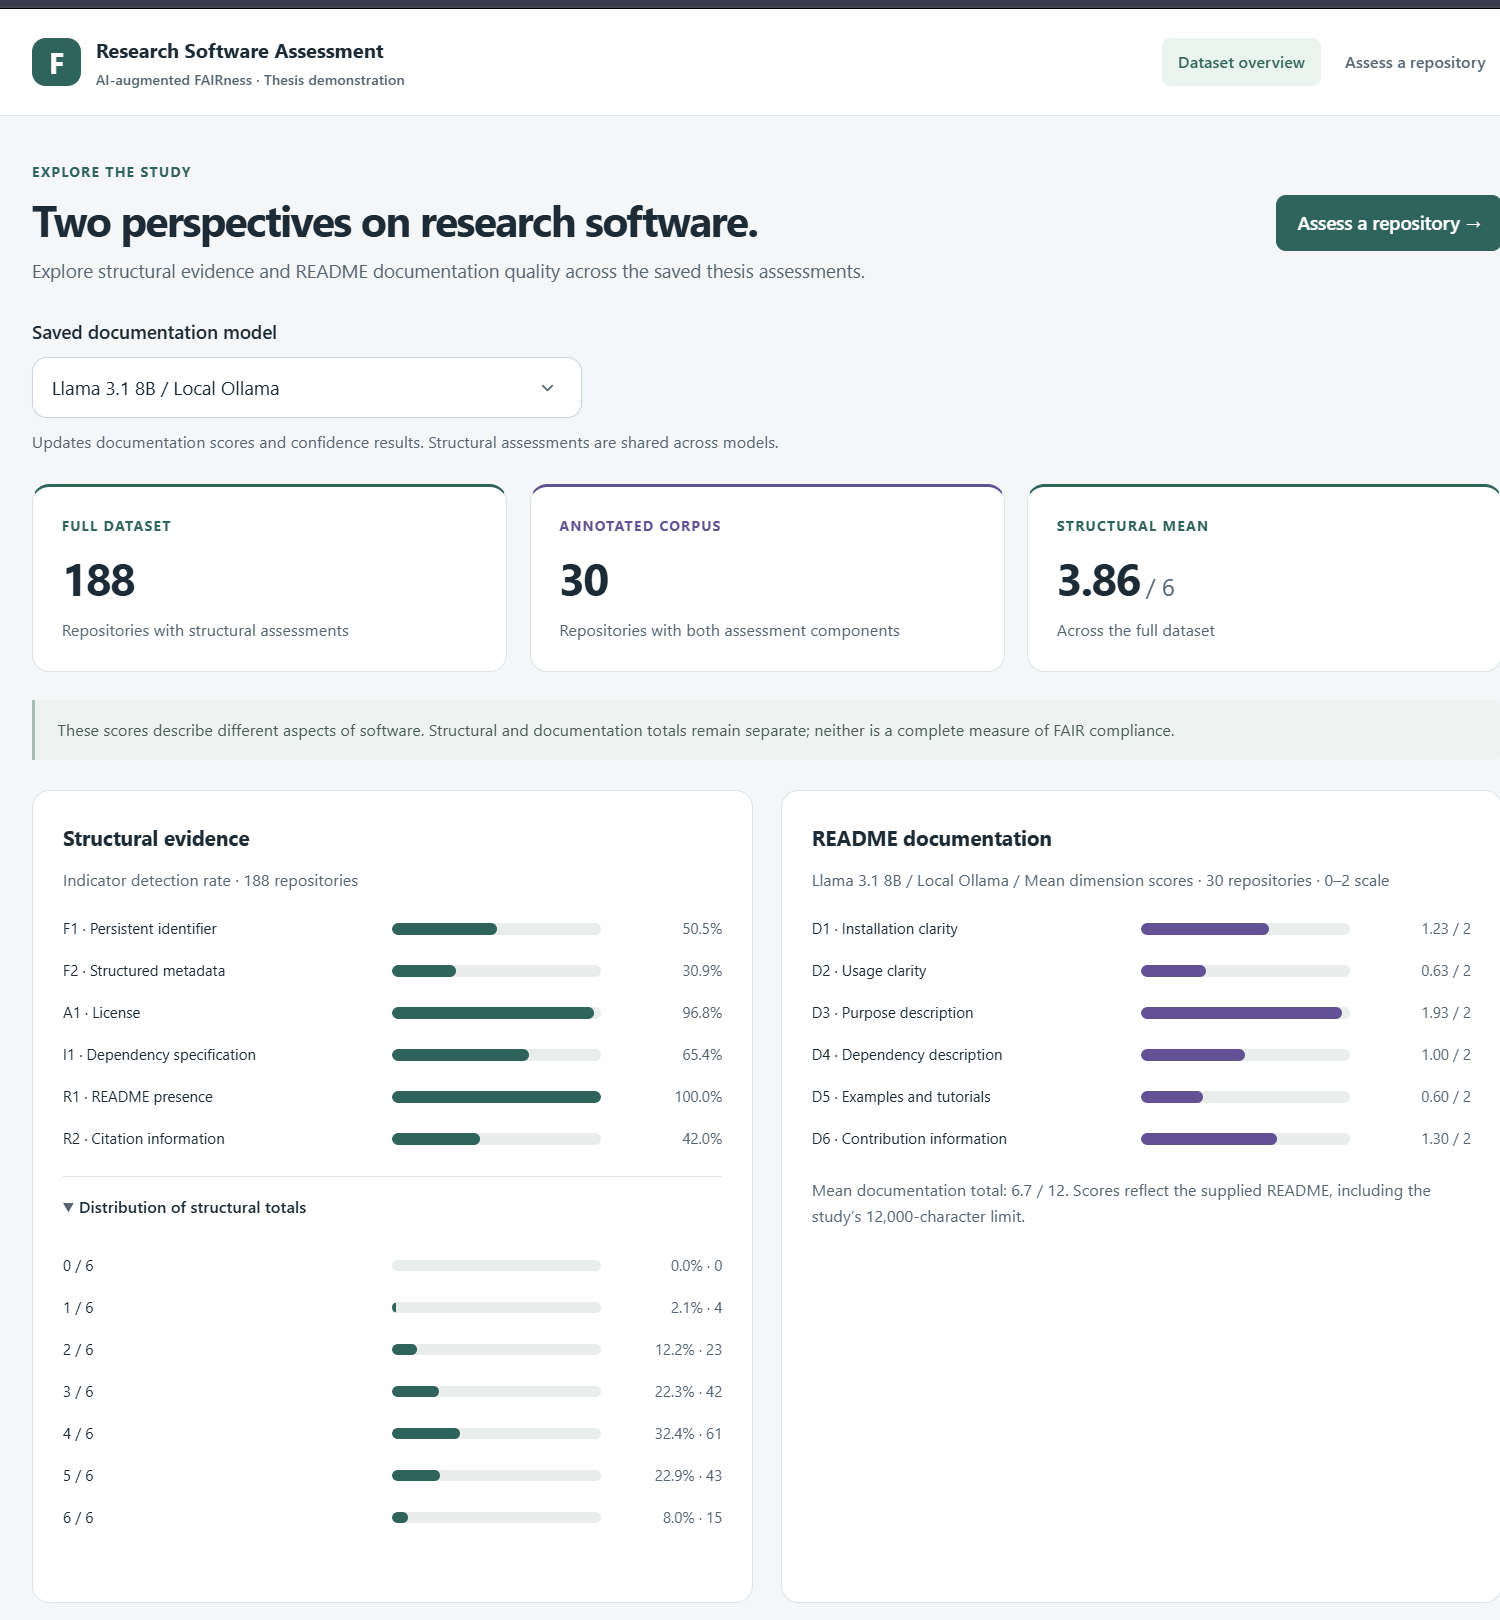
\includegraphics[
            width=\textwidth,
            height=0.36\textheight,
            keepaspectratio
        ]{figures/ui/web_overview_llama.png}
        \caption{Dataset overview with the saved Llama 3.1 8B assessment.}
        \label{fig:web_overview_llama}
    \end{subfigure}

    \vspace{0.7em}

    \begin{subfigure}{\textwidth}
        \centering
        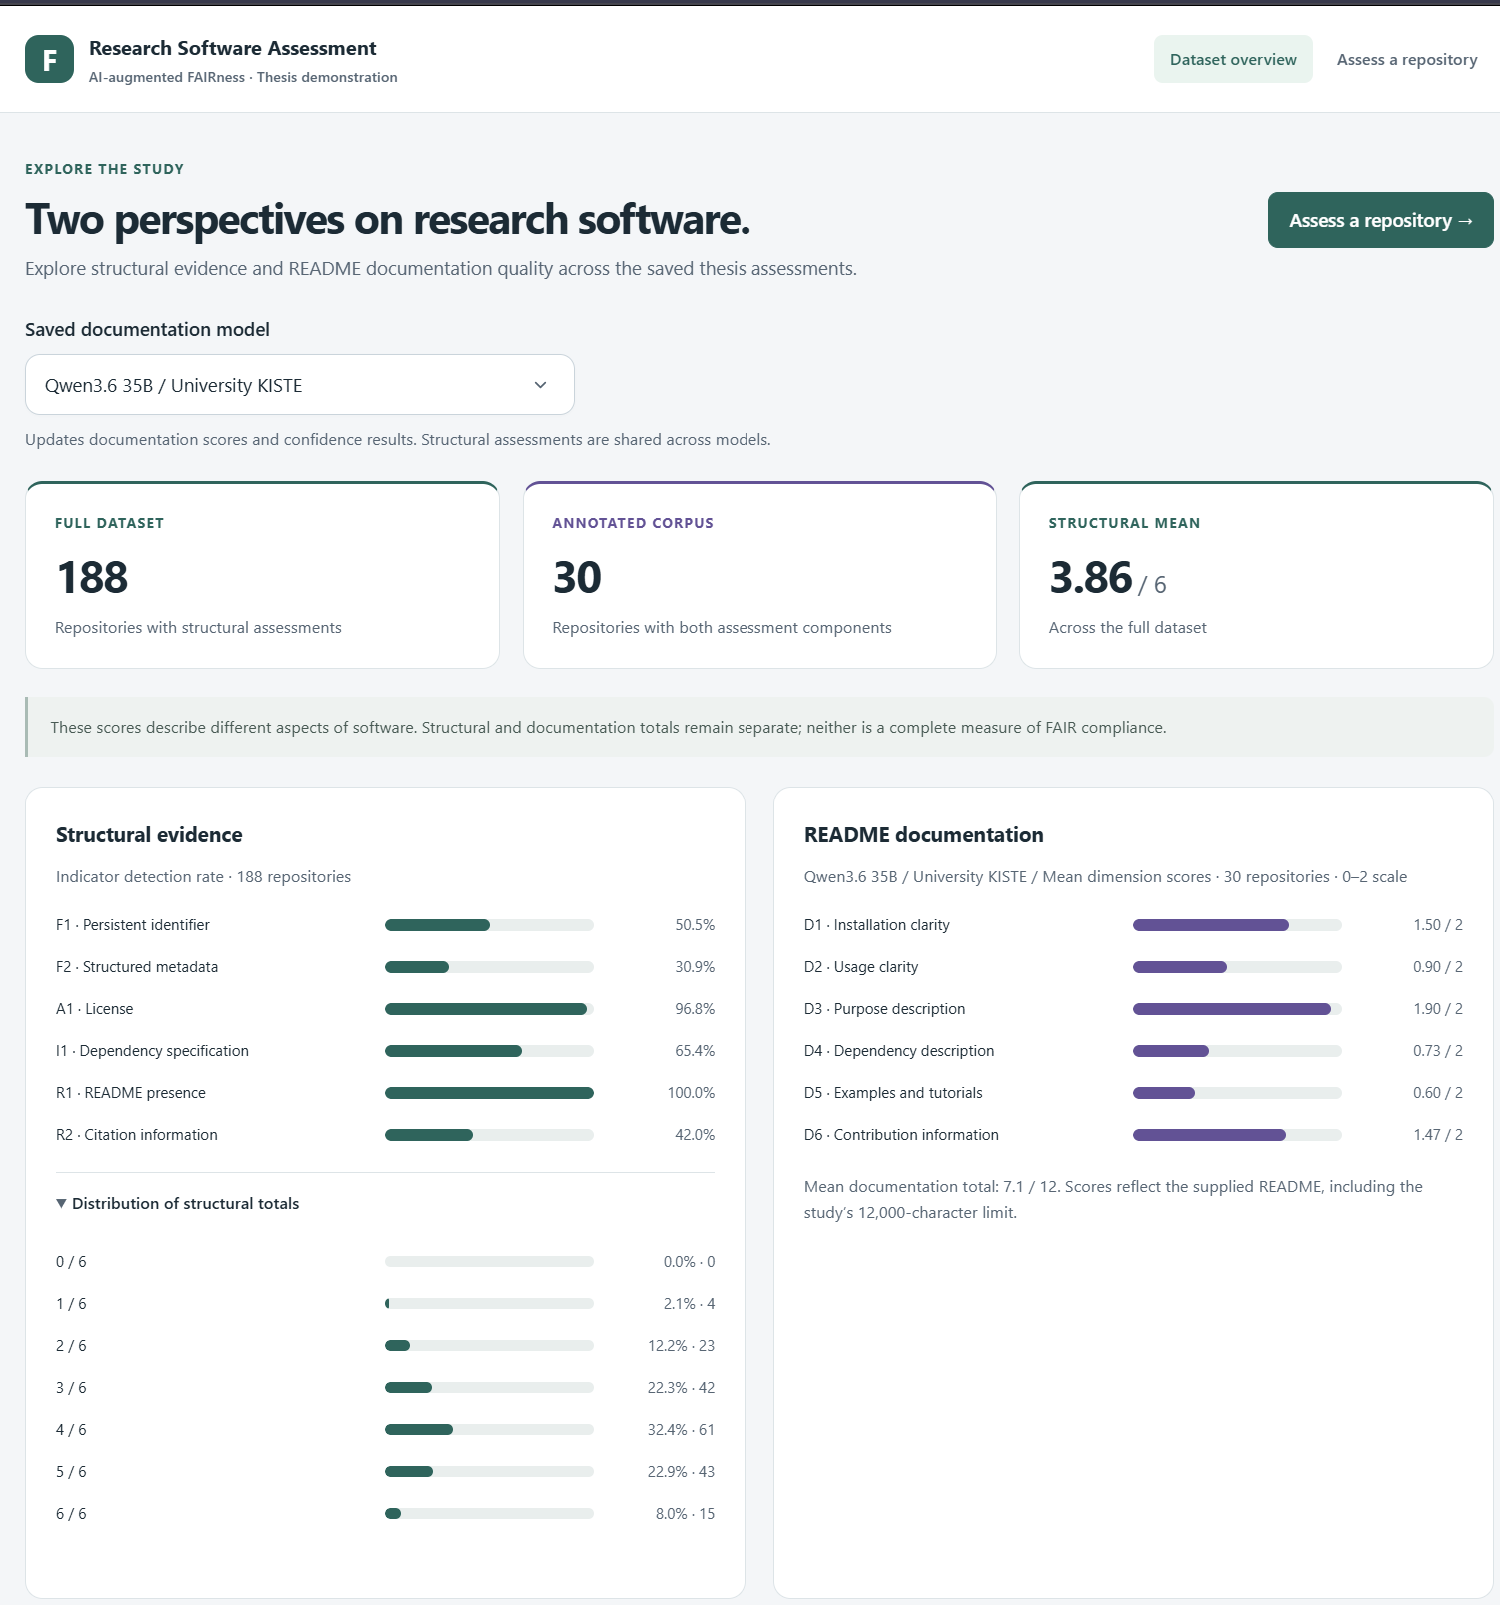
\includegraphics[
            width=\textwidth,
            height=0.36\textheight,
            keepaspectratio
        ]{figures/ui/web_overview_qwen.png}
        \caption{Dataset overview with the saved Qwen assessment.}
        \label{fig:web_overview_qwen}
    \end{subfigure}

    \caption{Dataset overview of the web-based assessment interface for
    the two evaluated documentation models. Structural evidence is shared
    across model selections, while the README documentation summaries
    reflect the selected LLM configuration.}
    \label{fig:web_overview}
\end{figure}

\FloatBarrier

\subsection{Research Evaluation View}

The web interface exposes selected evaluation results used to assess
the reliability of the implemented framework. The evaluation view
separates validation of the deterministic structural component from
analysis of the LLM-based documentation component.

For the structural component, precision, recall, and F1-score are
presented for each of the six binary indicators against the manually
annotated 30-repository corpus. The interface additionally reports the
corresponding results for the 20-repository pilot-exclusion subset.
This latter analysis is explicitly identified as an internal
consistency check rather than as independent validation, since some
annotations in this subset were corrected during scorer validation
using the finalized rubric.

For the documentation component, the interface provides two forms of
evaluation information. First, model-reported confidence labels are
shown together with exact agreement, mean absolute error, and weighted
Cohen's Kappa against the human reference annotations. The interface
explicitly states that these confidence labels are self-reported and
should not be interpreted as calibrated probabilities of correctness.

Second, an interactive agreement view allows the two evaluated LLM
configurations to be compared against either the primary or second
human annotator. The user can inspect results for the complete
30-repository annotated corpus or exclude the ten pilot repositories
to obtain the 20-repository pilot-exclusion sensitivity analysis.
For each model, the interface reports mean weighted Cohen's Kappa,
exact agreement, and mean absolute error, together with corresponding
per-dimension results for D1--D6. Higher documentation scores are not
presented as evidence of better model performance; agreement is
evaluated relative to the selected human reference.

Figures~\ref{fig:web_evaluation_validation} and
\ref{fig:web_evaluation_agreement} illustrate these two parts of the
research evaluation interface. The methodology and interpretation of
the displayed results are discussed in Chapter~5.

\begin{figure}[p]
    \centering
    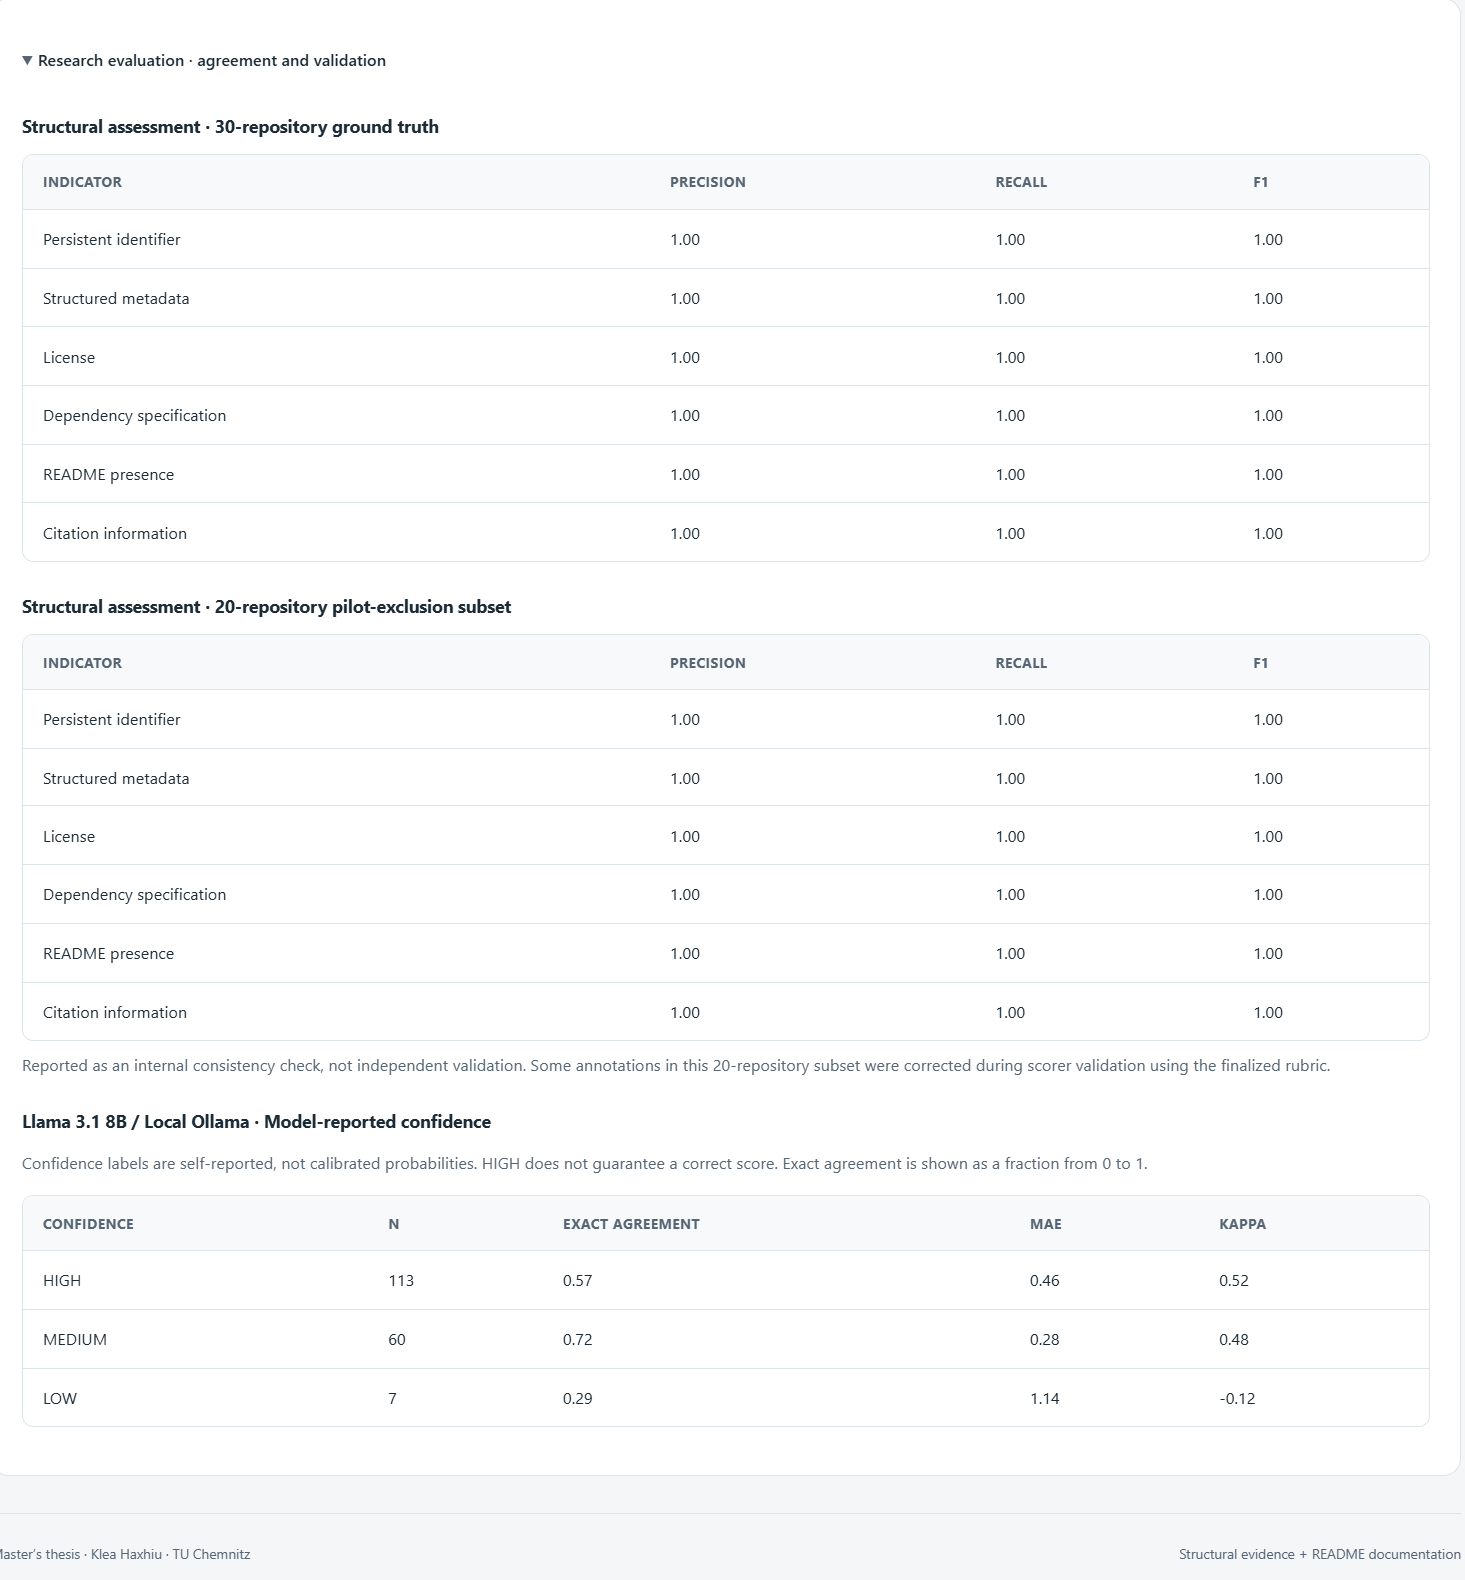
\includegraphics[
        width=\textwidth,
        height=0.78\textheight,
        keepaspectratio
    ]{figures/ui/web_structural_validation_confidence.png}
    \caption{Structural validation and confidence analysis in the
    research evaluation interface. The view reports precision, recall,
    and F1-score for the structural indicators on the annotated corpus
    and pilot-exclusion subset, together with model-reported confidence
    statistics for the documentation assessment.}
    \label{fig:web_evaluation_validation}
\end{figure}

\begin{figure}[p]
    \centering
    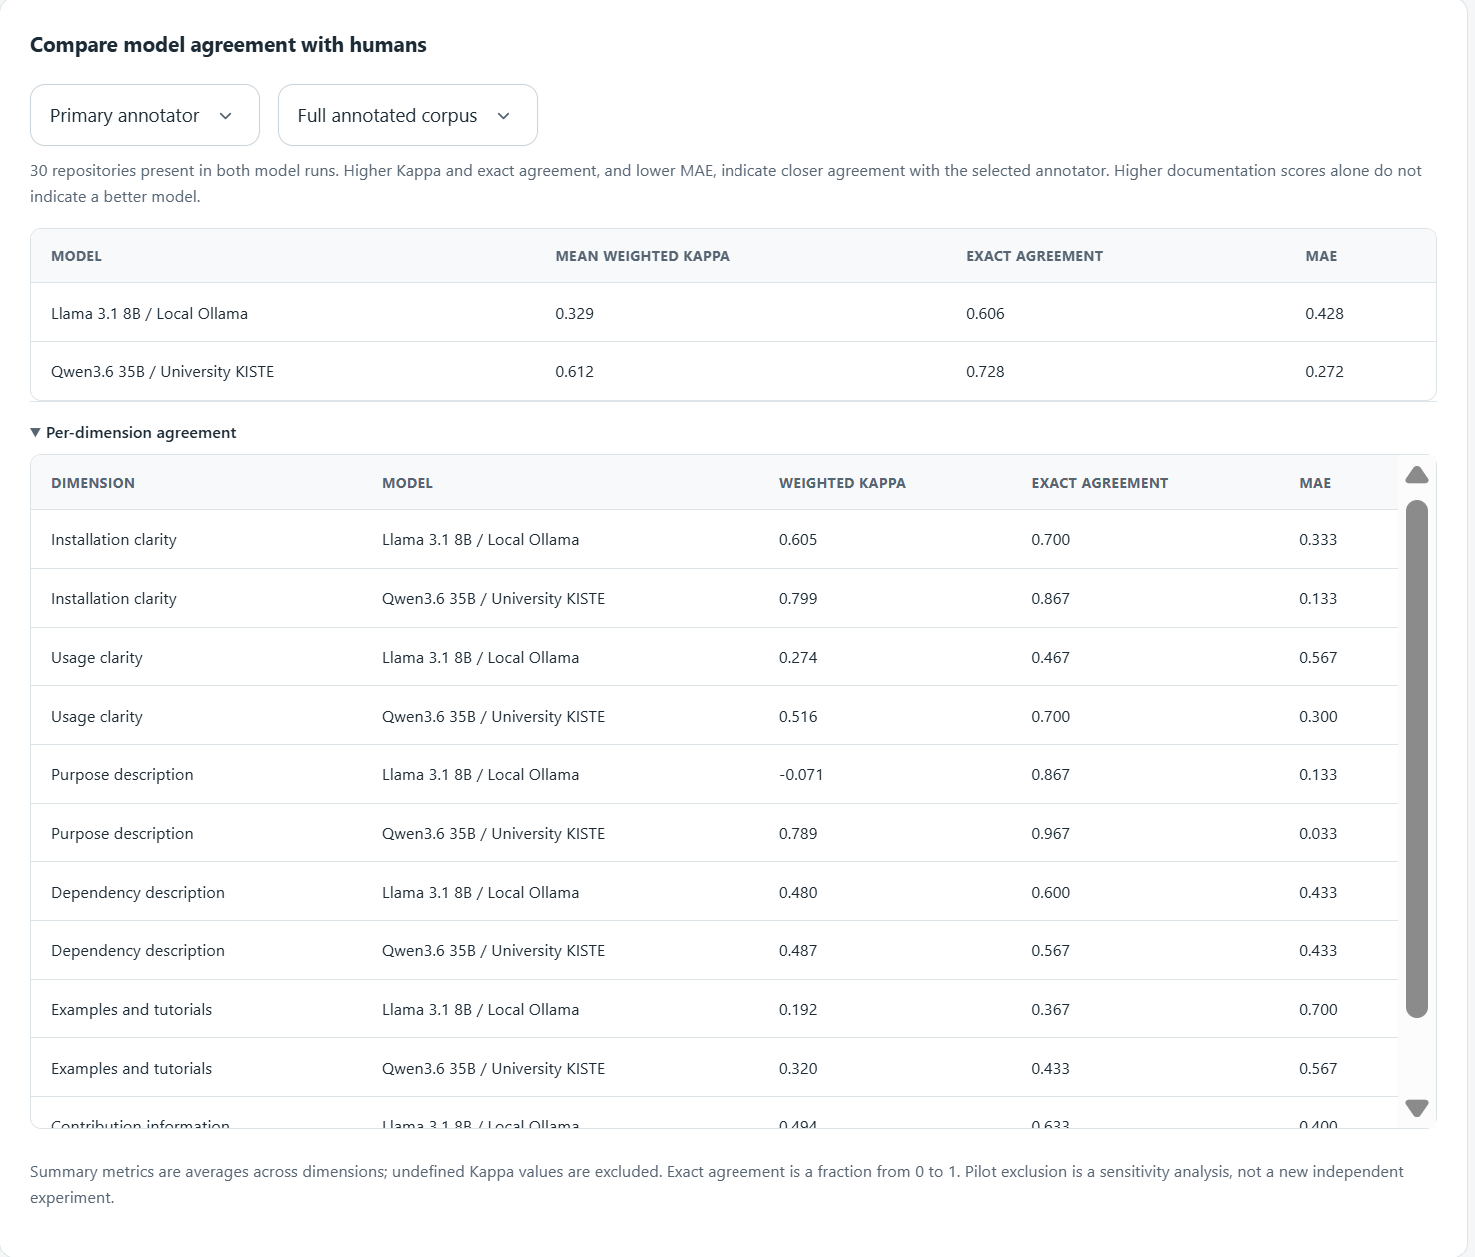
\includegraphics[
        width=\textwidth,
        height=0.78\textheight,
        keepaspectratio
    ]{figures/ui/web_evaluation_agreement.png}
    \caption{LLM--human agreement view for the annotated corpus. The
    interface compares the saved Llama and Qwen assessments against
    the selected human annotator using weighted Cohen's Kappa, exact
    agreement, and mean absolute error, with corresponding
    per-dimension results for D1--D6.}
    \label{fig:web_evaluation_agreement}
\end{figure}

\FloatBarrier


\subsection{Model Comparison View}

For repositories in the annotated evaluation corpus, the prototype
provides a side-by-side comparison of the saved Llama and Qwen
documentation assessments. The comparison presents the D1--D6 scores
from both model configurations together with the selected human
reference annotations and highlights dimensions on which the model
outputs differ.

This functionality is intended primarily to support transparent
inspection of model-dependent assessment behaviour rather than to
present the two configurations as interchangeable user preferences.
The comparison operates exclusively on the saved experimental results
and does not trigger new LLM inference. Model identifiers, reasoning
statements, and confidence labels remain visible so that differences
can be traced to the corresponding assessment output.

Figure~\ref{fig:web_model_comparison} shows the model-comparison view
for a repository from the annotated corpus.

\begin{figure}[p]
    \centering
    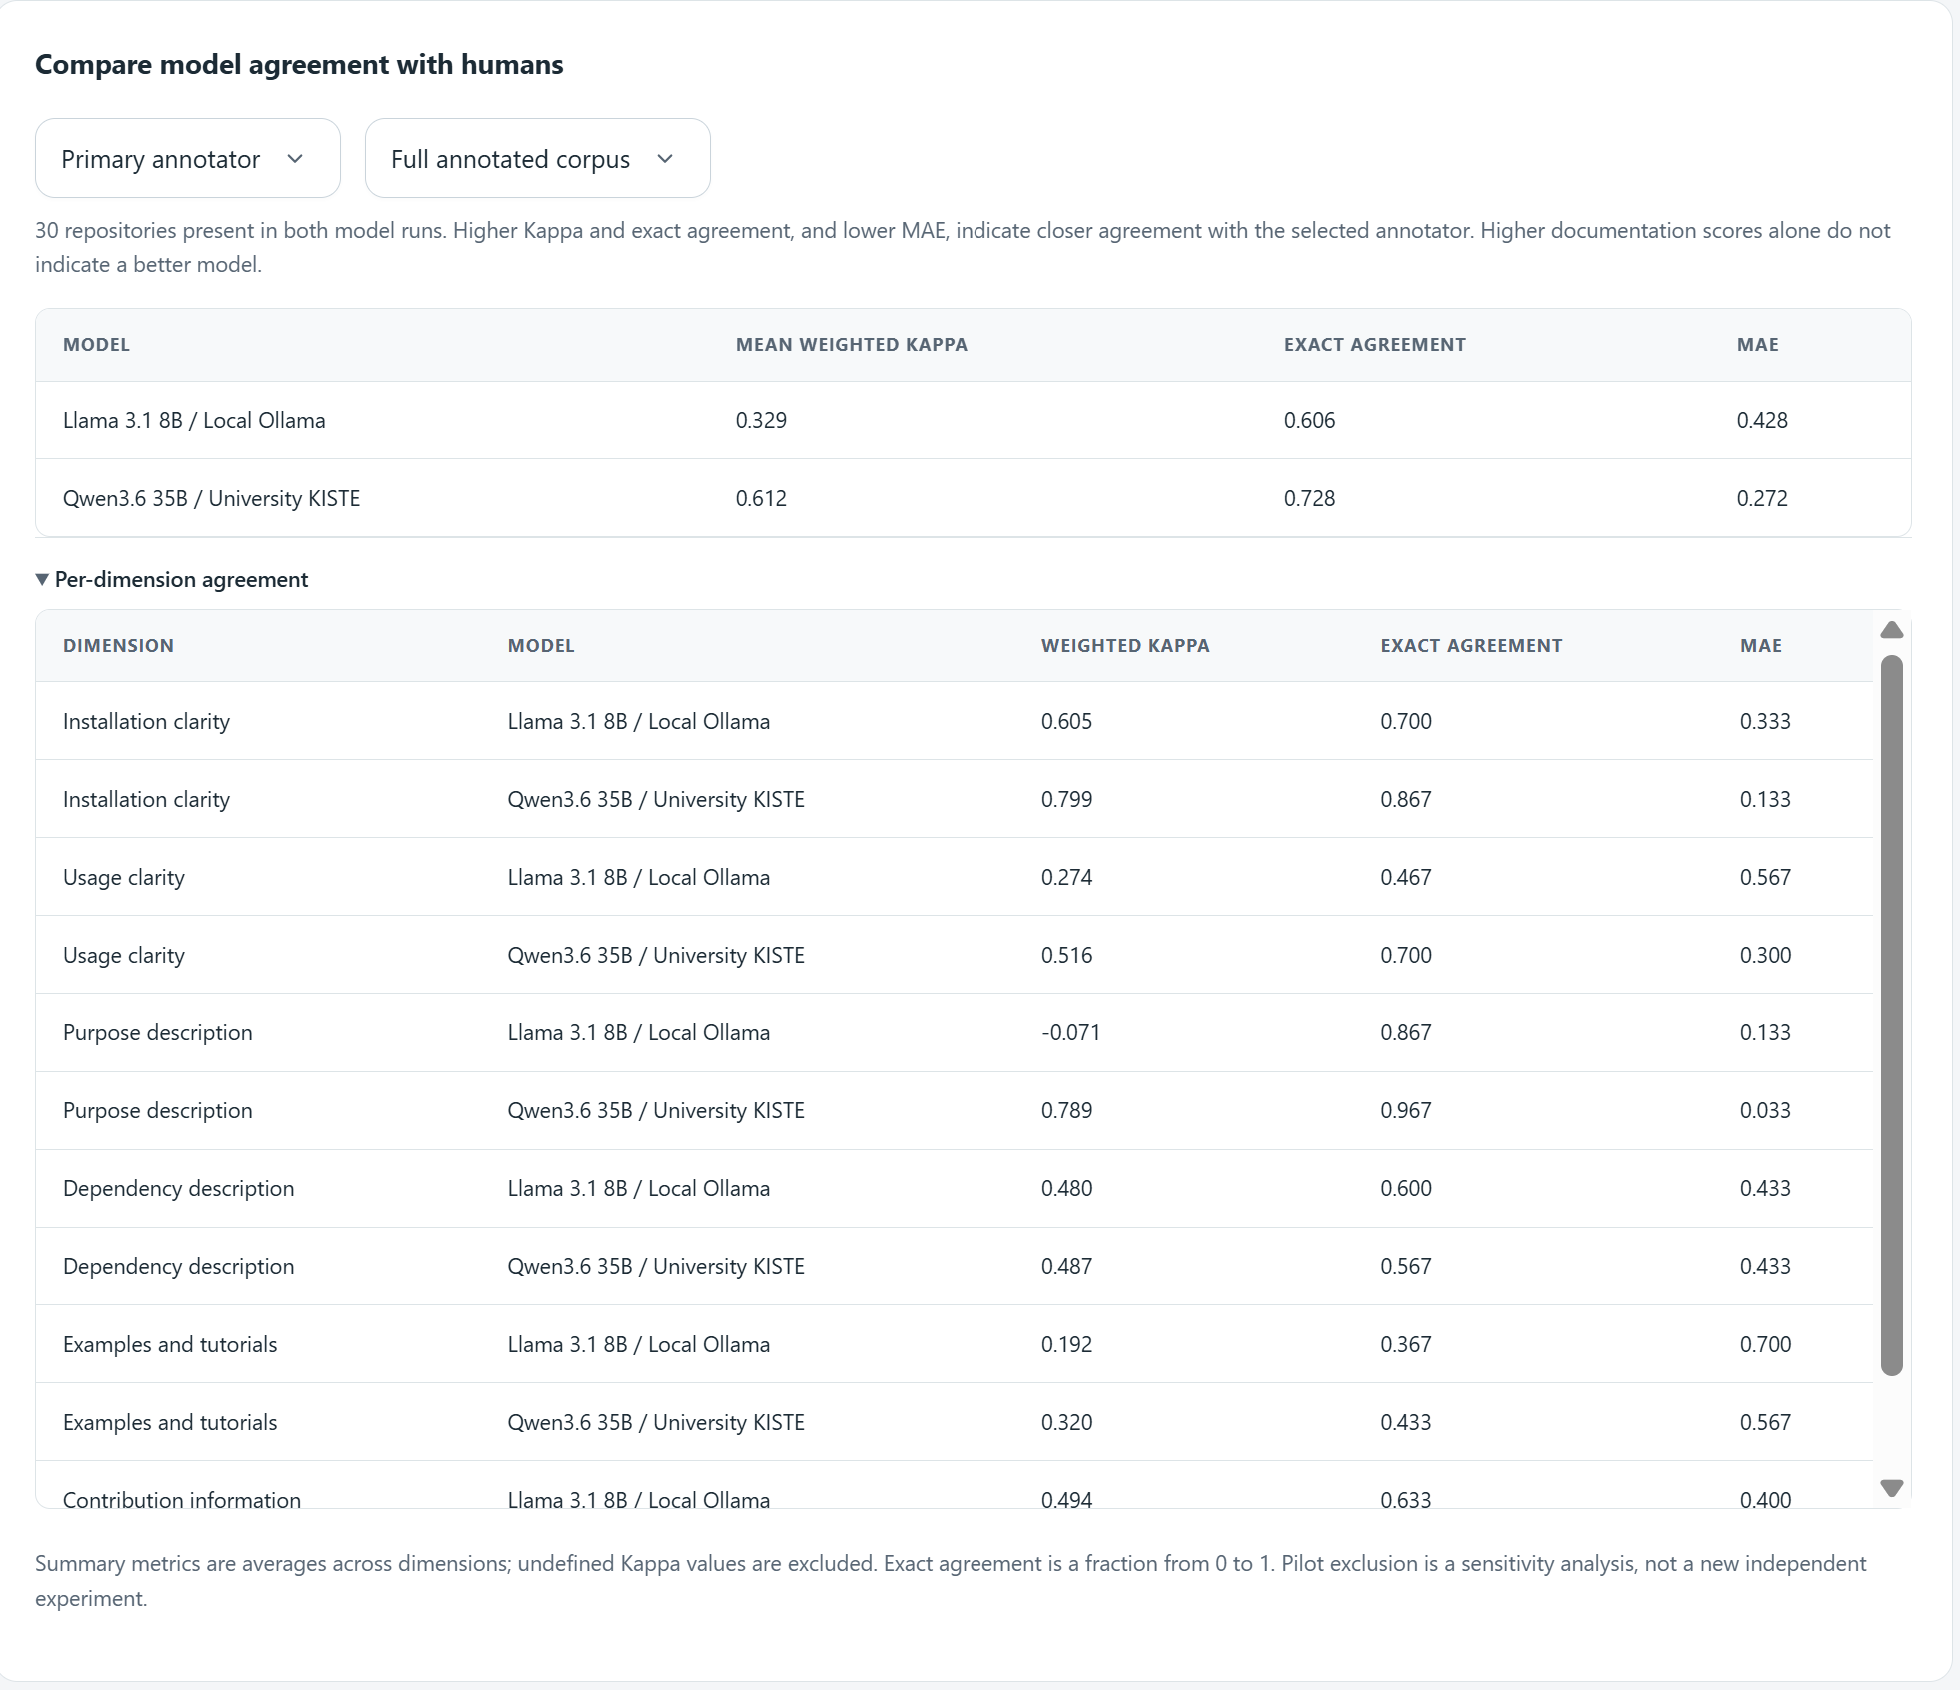
\includegraphics[
        width=\textwidth,
        height=0.78\textheight,
        keepaspectratio
    ]{figures/ui/web_model_comparison.png}
    \caption{Model-comparison view for a repository in the annotated
    corpus. Saved Llama and Qwen documentation assessments are shown
    alongside the selected human reference scores, allowing
    model-dependent differences across D1--D6 to be inspected.}
    \label{fig:web_model_comparison}
\end{figure}

\FloatBarrier

\subsection{Repository Browser}

The web interface includes a searchable repository browser that
provides access to the saved assessment results. Users can search by
repository owner or name and switch between the annotated corpus and
the full repository dataset.

For the annotated corpus, the browser contains the 30 repositories for
which both structural and LLM-based documentation assessments are
available. The documentation totals shown in this view correspond to
the currently selected LLM configuration, while the structural results
remain unchanged because they are independent of the selected model.
Repository entries provide access to the corresponding model-specific
saved report and, where both model outputs are available, to the
model-comparison view.

In contrast, the full-dataset view contains all 188 repositories for
which the structural assessment was executed. Since the LLM-based
assessment was not executed across this complete dataset, the
documentation field is shown as ``Not assessed'' rather than assigning
a documentation score of zero.

Selecting ``View report'' opens the repository-level assessment view,
where the individual structural indicators and, where available,
documentation dimensions and supporting assessment information can be
inspected. An example of this detailed view is presented in the
following subsection using \texttt{astropy/astropy}.

Figure~\ref{fig:web_repository_browser} shows the two repository-browser
cohorts exposed by the interface. The annotated-corpus view provides
access to the hybrid profiles for the 30 repositories with both
assessment components, whereas the full-dataset view exposes the
structural assessments for all 188 repositories and explicitly marks
documentation as not assessed where no LLM assessment was performed.

\begin{figure}[p]
    \centering

    \begin{subfigure}{\textwidth}
        \centering
        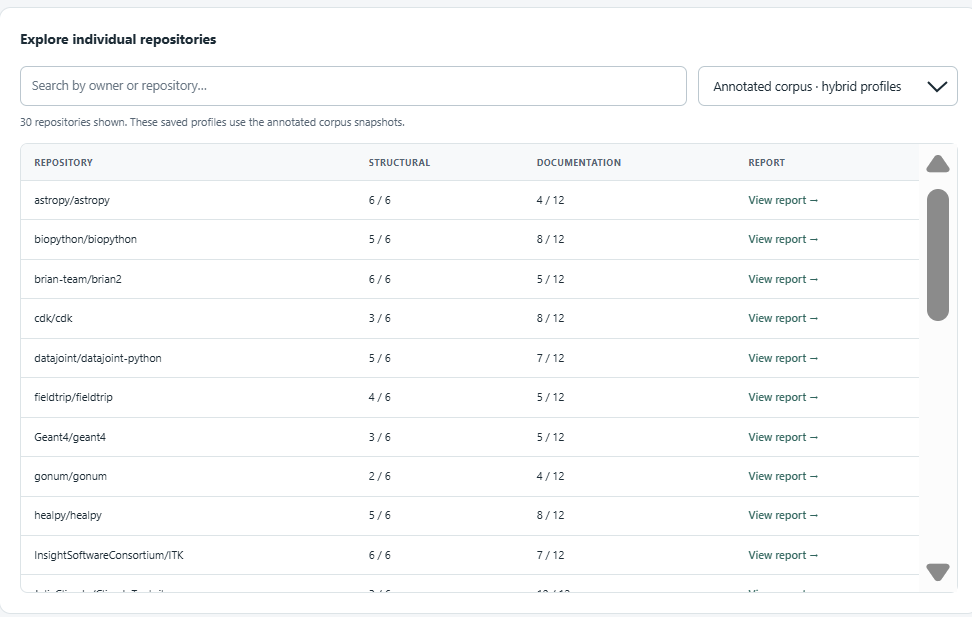
\includegraphics[
            width=\textwidth,
            height=0.36\textheight,
            keepaspectratio
        ]{figures/ui/web_browser_annotated.png}
        \caption{Annotated corpus with hybrid profiles.}
        \label{fig:web_browser_annotated}
    \end{subfigure}

    \vspace{0.7em}

    \begin{subfigure}{\textwidth}
        \centering
        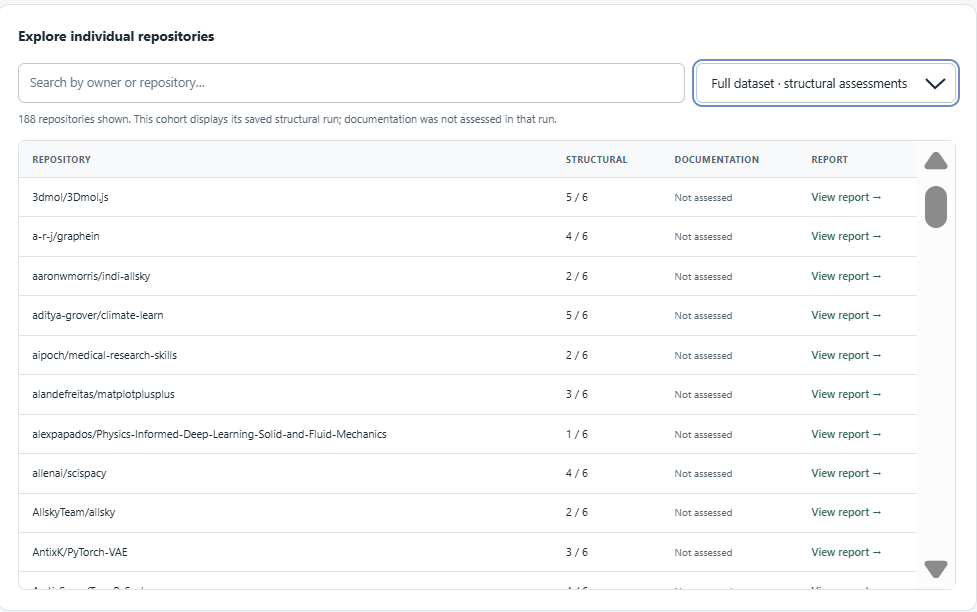
\includegraphics[
            width=\textwidth,
            height=0.36\textheight,
            keepaspectratio
        ]{figures/ui/web_browser_full.png}
        \caption{Full dataset with structural assessments only.}
        \label{fig:web_browser_full}
    \end{subfigure}

    \caption{Repository browser for the two saved assessment cohorts.
    (a) The 30-repository annotated corpus exposes structural and
    model-specific documentation results together with access to model
    comparison. (b) The full 188-repository dataset exposes the saved
    structural assessments, while documentation is marked as not assessed
    because LLM-based assessment was not executed for this cohort.}
    \label{fig:web_repository_browser}
\end{figure}

\FloatBarrier
\subsection{Repository-Level Assessment View}

Individual saved assessments can also be inspected through a
repository-level view. This view presents the six structural indicators
and six documentation dimensions as separate components of the hybrid
profile. Documentation dimensions can be expanded to inspect the
reasoning produced by the LLM, its model-reported confidence label, and
the rubric associated with the corresponding score.

Saved documentation assessments are model-specific. Selecting a
different LLM configuration loads the corresponding persisted
documentation scores, reasoning, confidence labels, and assessment
metadata, while the deterministic structural component remains
unchanged.

The interface additionally exposes the README evidence and assessment
metadata, including the result source, model, and assessment timestamp.
This provides a transparent presentation of the evidence underlying an
assessment rather than exposing only the resulting numerical scores.

Figure~\ref{fig:web_repository} shows the saved assessment for
\texttt{astropy/astropy}, corresponding to the example profile
presented in the preceding section.

\begin{figure}[p]
    \centering
    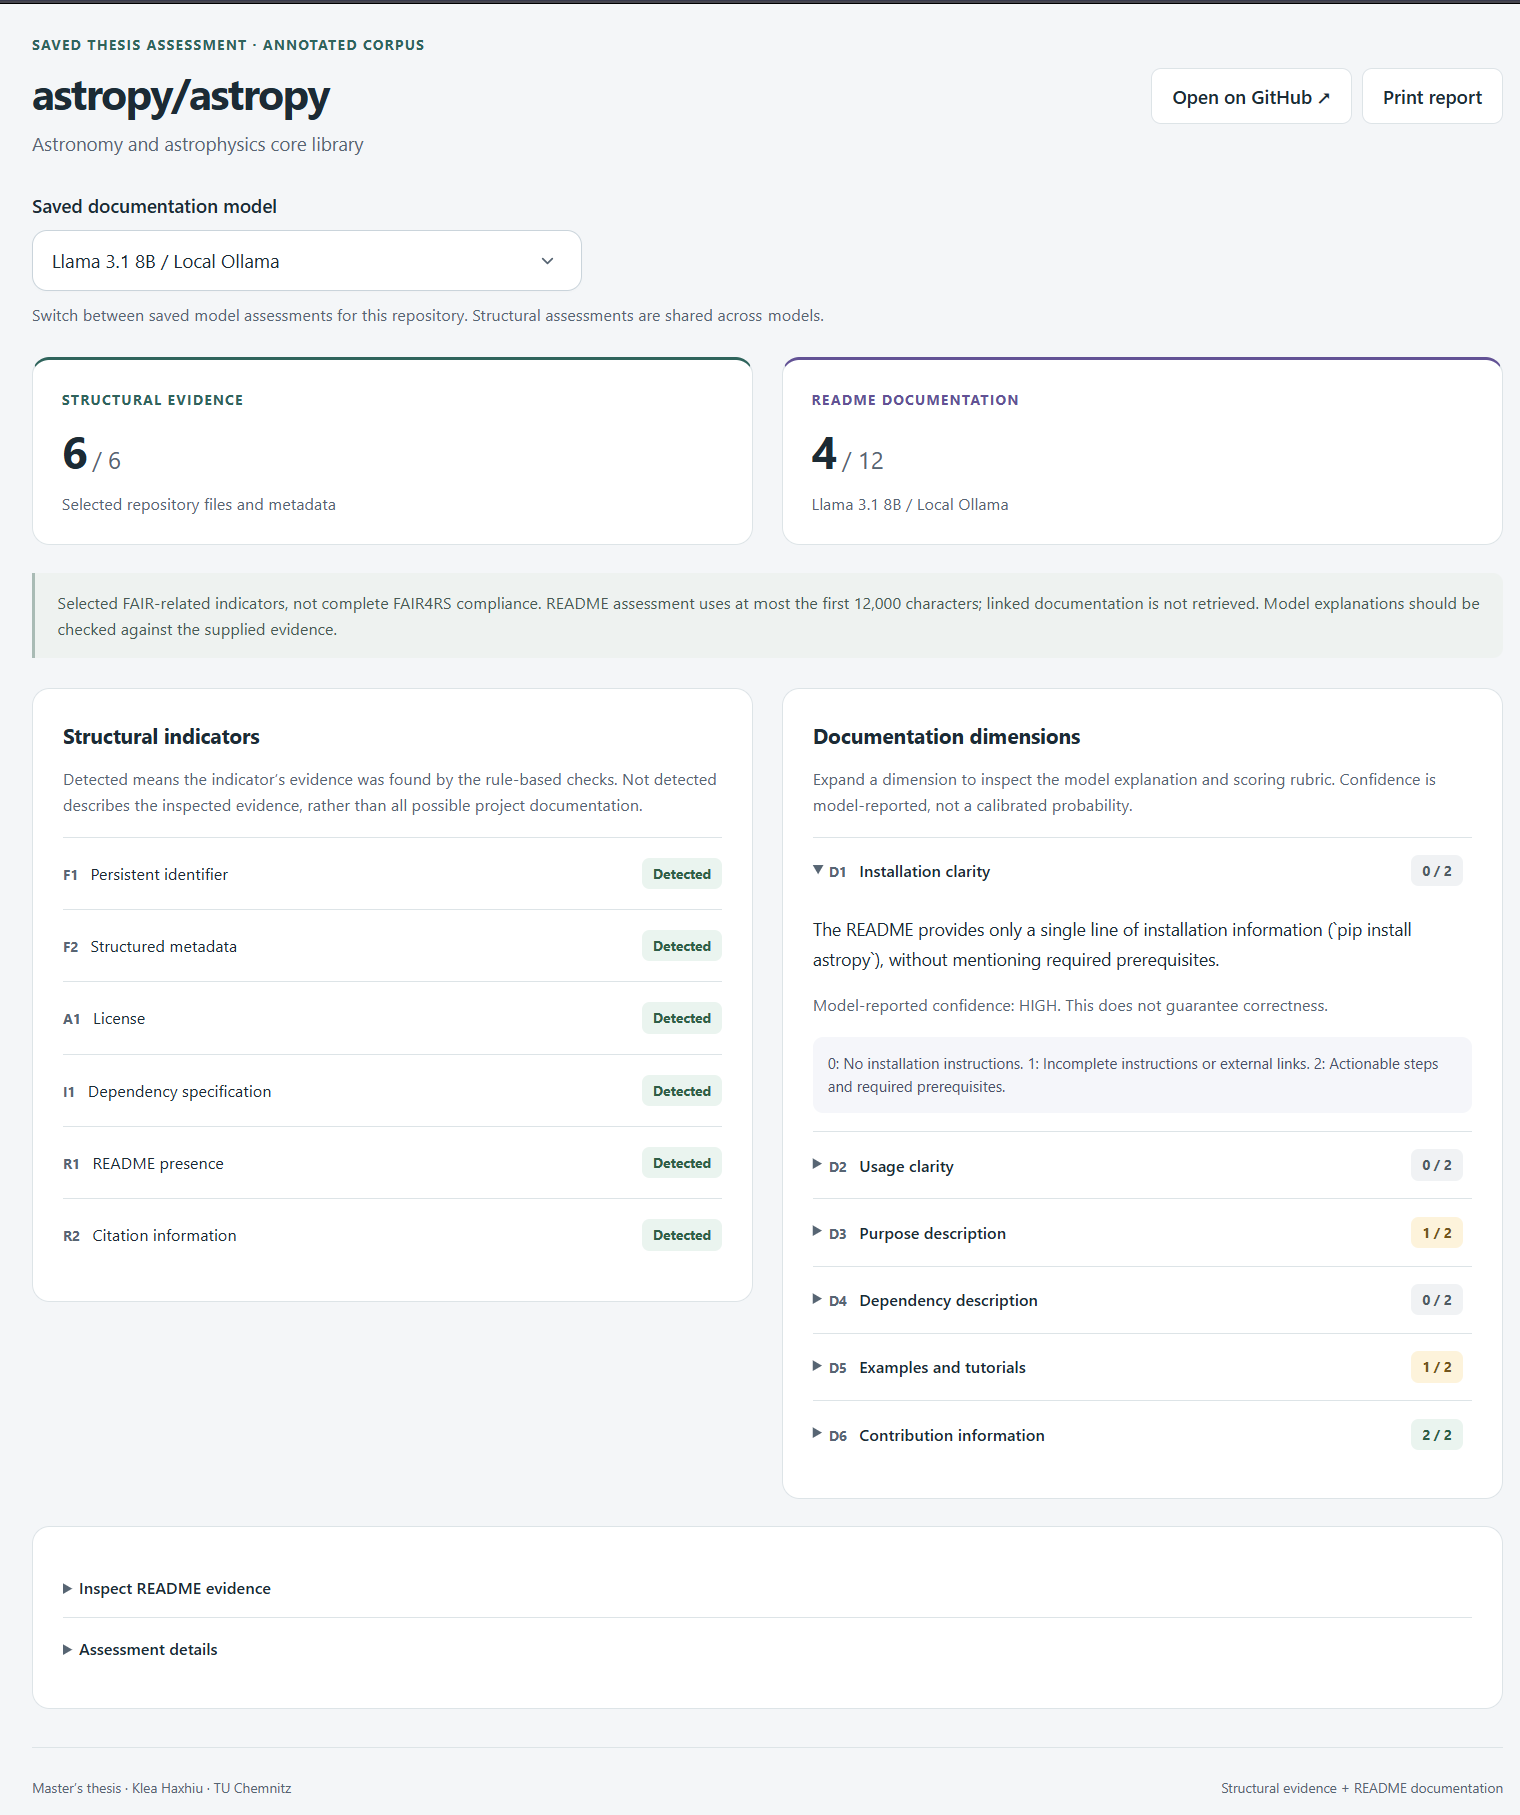
\includegraphics[
        width=\textwidth,
        height=0.78\textheight,
        keepaspectratio
    ]{figures/ui/web_repository_llama.png}
    \caption{Repository-level hybrid assessment for
    \texttt{astropy/astropy}. The interface presents deterministic
    structural indicators and the documentation assessment for the
    selected LLM configuration as separate components. Documentation
    dimensions can be expanded to inspect model-generated reasoning,
    reported confidence, and the scoring rubric, while the underlying
    README evidence and assessment metadata remain available for
    inspection.}
    \label{fig:web_repository}
\end{figure}

\FloatBarrier

\subsection{Live Repository Assessment}

In addition to inspecting saved thesis results, the prototype supports
assessment of a newly supplied public GitHub repository. The user
provides a repository identifier or GitHub URL and can request the
optional README documentation assessment. The backend retrieves the
current repository evidence and applies the same structural checks used
by the batch pipeline. 
When documentation assessment is enabled, the user can select the LLM
configuration used for the live assessment. Llama~3.1~8B is accessed
through the local Ollama service, whereas
\texttt{Qwen3.6-35B-A3B-MLX-8bit} is accessed through the university
KISTE service. The selected provider is handled by the backend, and
service availability or inference failures are reported explicitly
without discarding successfully computed structural results.

The resulting view preserves the same distinction between structural
and documentation-based assessment used for saved profiles. Each
documentation dimension can be expanded to inspect its score,
reasoning, confidence label, and rubric. Because these assessments
operate on current GitHub content, their results may differ from
previously collected repository snapshots. They are therefore treated
as interactive prototype results and remain separate from the fixed
experimental datasets used in Chapter~5.

As an implementation-level verification of the remote provider path, a
live assessment was successfully completed using the Qwen configuration
through the university KISTE service. This exercised the complete path
from retrieval of current GitHub repository evidence through remote LLM
inference and response validation to presentation of the resulting
hybrid profile. This verification concerns the operation of the web
prototype and is separate from the fixed experimental Qwen evaluation
reported in Chapter~5.

Figure~\ref{fig:web_live} shows a completed live assessment of
\texttt{pandas-dev/pandas}.

\begin{figure}[p]
    \centering
    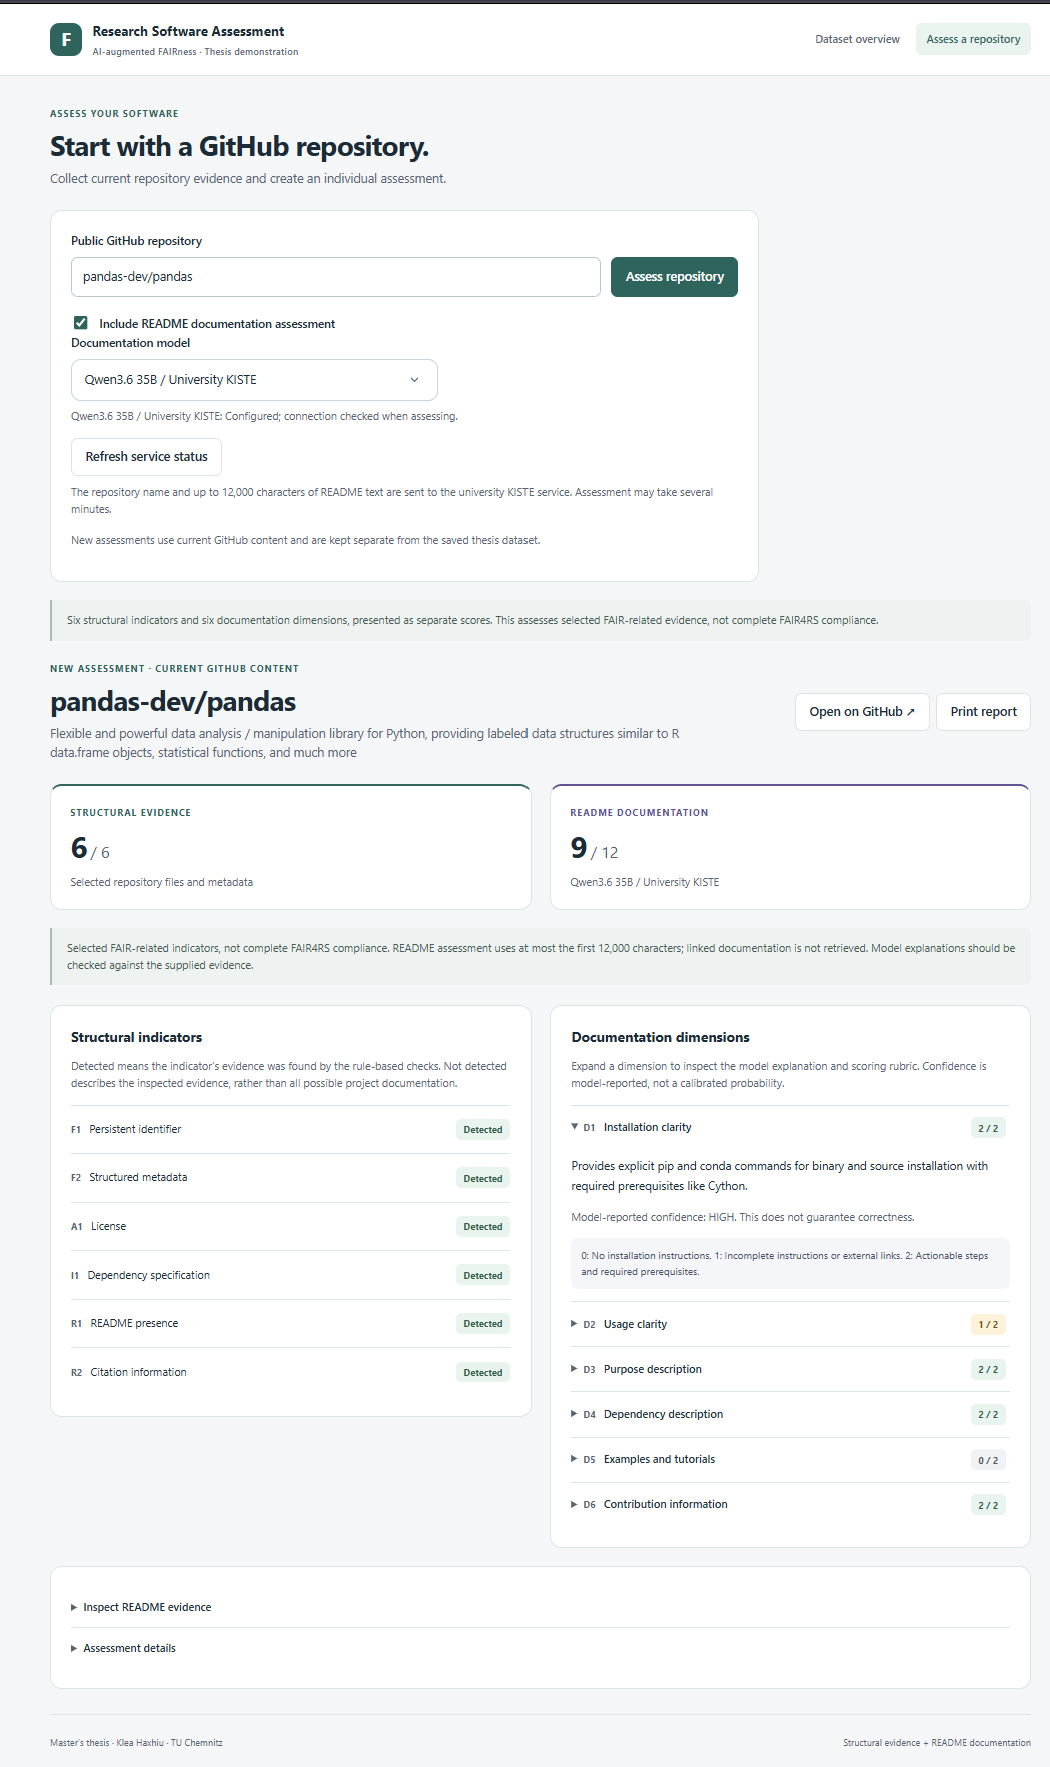
\includegraphics[
        width=\textwidth,
        height=0.78\textheight,
        keepaspectratio
    ]{figures/ui/web_live_qwen.png}
    \caption{Completed live assessment of \texttt{pandas-dev/pandas} using
the Qwen configuration through the university KISTE service. The
prototype retrieves current GitHub evidence, applies the deterministic
structural checks, and performs the optional README documentation
assessment. Structural and documentation scores remain separate, and
individual documentation dimensions expose the model-generated
reasoning, reported confidence, and scoring rubric.}
\label{fig:web_live}
\end{figure}

\FloatBarrier
\subsection{Implementation Limitations}

The web prototype inherits the evidence boundaries of the underlying
assessment pipeline. The qualitative component evaluates README
content only and does not retrieve documentation behind external
links. README input to the LLM is subject to the same 12{,}000-character
limit described in Chapter~3. Consequently, a live assessment should
be interpreted as an assessment of the evidence available to the
implemented framework rather than as a complete evaluation of all
documentation associated with a software project.

Live repository assessment additionally depends on access to GitHub,
while live documentation scoring depends on the selected LLM
provider. Llama assessment requires a configured local Ollama
instance, whereas Qwen assessment requires access to the university
KISTE service and a server-side authentication token. Authentication
credentials are not exposed to the frontend. Provider unavailability
or inference failure is reported to the user while preserving any
structural assessment that was successfully completed.
Model-reported confidence is displayed as contextual information and
is not presented as a calibrated probability of correctness.

\section{Implementation Summary}

This chapter has described the implementation of the proposed hybrid
FAIRness assessment framework. Its core assessment pipeline consists
of repository data collection, a rule-based assessment component, an
LLM-based documentation assessment component, and hybrid profile
generation. Repository data and assessment outputs are persisted using
local JSON and CSV files, allowing individual processing stages and
their underlying evidence to be inspected and re-run independently.

The documentation component supports two evaluated model
configurations: Llama~3.1~8B through local Ollama and
\texttt{Qwen3.6-35B-A3B-MLX-8bit} through the university KISTE
service. Model-specific documentation results are retained separately
and combined with the shared deterministic results without reducing
the two assessment components to a single score.

A web-based prototype was additionally implemented on top of the
assessment pipeline to make the resulting assessments directly
inspectable and to support assessment of newly supplied public GitHub
repositories. The interface exposes aggregate dataset summaries,
model-specific evaluation results, searchable access to saved
repository assessments, side-by-side comparison of the two LLM
configurations against human reference annotations, repository-level
hybrid profiles, underlying assessment evidence, model-generated
reasoning and confidence information, and live repository assessment
using either supported LLM provider.

Saved experimental results remain separated from live assessments so
that interactive use of the prototype does not modify the fixed
datasets evaluated in the following chapter. Throughout the interface,
structural and documentation-based results remain separate, preserving
the hybrid design of the proposed framework.

The following chapter evaluates the accuracy and reliability of the
assessment components against the manually annotated ground truth,
examines differences between the two evaluated LLM configurations, and
compares the proposed approach with existing FAIR assessment tools.